\section{ps4: Checkers}\label{sec:ps4}

\subsection{Overview}\label{sec:ps4:overview} % A discussion of the assignment itself

This project builds the widely known game of Checkers.
In this game, two players, black and red, look to remove each other's pieces by jumping over them.
When a player no longer ahs any piece on the game board the other player wins. 
During a player's turn they can select a piece and it will highlight the tiles where the piece can move.
A piece can move in two diagonal directions depending on the piece's color.
If that move includes jumping a piece, the piece that is jumped is removed from the game board.
If a piece arrives at the opposing players side that piece is 'kinged', and can now move in all four diagonal directions. 
The game mechanics that were not yet implemented were multi-jumping, and forcing a player to make a jump if they can.

\subsection{End Product}\label{sec:ps4:accomplish} % What I accomplished and images/results

Below is the output.
This is the standard setup for a Checkers game.

\begin{figure}[h]
\centering
\begin{minipage}[b]{0.4\textwidth}
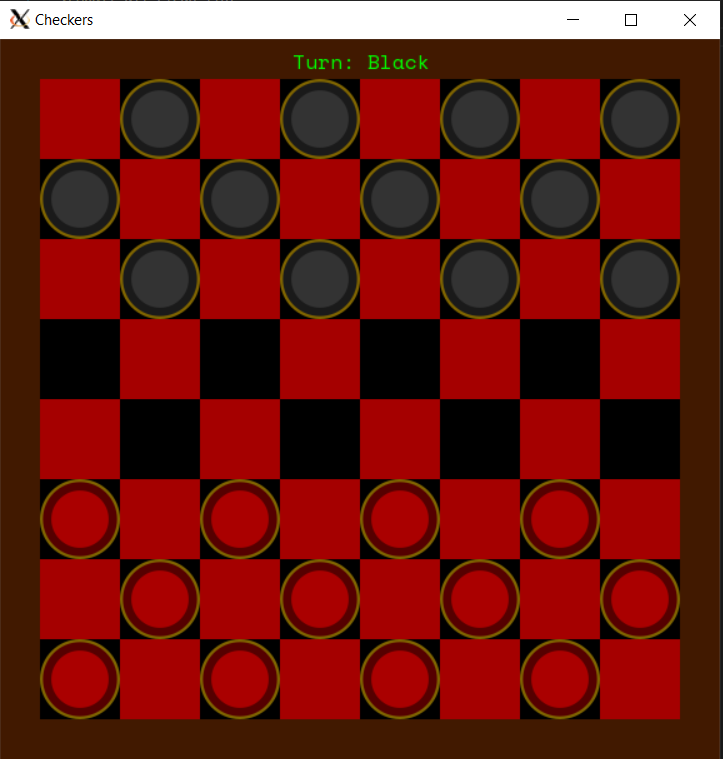
\includegraphics[width=\textwidth]{ps4-1_output}
\caption{Checkers: Start}
\end{minipage}
\end{figure}

\subsection{What I Already Knew}\label{sec:ps4:knew} % What was known prior to the assignment

Going into this project I had already completed Sokoban, so I had a good foundation for creating a game UI in SFML and implementing its game mechanics using C++.

\subsection{Design Decisions and Implementations}\label{sec:ps4:decisions} % Important decisions or implementations I made

The code for Checkers was comprised of two major classes called 'Checkers' and 'Pawn'.
The 'Pawn' class was meant to represent a piece and contained the sprite for a game piece along with a boolean that indicated if it was a king or not.
In the 'Checkers' class I made a a vector containing the game textures with similar reasoning to the textures vector in Sokoban.
The game tiles were represented using a 2d-vector of rectangles.
Each player's peieces were separated into their own respective vectors of 'Pawns', one representing the red player and the other the black.
The Checkers class also had a boolean variable named '\_blackTurn' to represent whose turn it was.

The game starts by creating a 'Checkers' object which does the following:
\begin{itemize}
\item Creates a base layer of brown which represents the board's border.
\item Fills the 2d-vector of tiles with alternated red and black squares.
\item Adds a black piece to its respective vector for every black square that was in the first three rows and adds a red piece to its respective vector for every red piece that was in the final three rows.
\end{itemize}

Once the game was made a number of smaller helper functions were made to reduce repeat code and code length.
Here are some of the more important ones:
\begin{itemize}
\item 'isBlackTurn' - Returns whose turn it is, black or red.
\item 'toTile' - Converts a pixel's coordinates to a tile location.
\item 'inBounds' - Checks if a piece's move is in bound.
\item 'getCurrPieces' \& 'getOppPieces' - Returns the current players pieces and the opposing players pieces depending on whose turn it is.
\item 'clearHighlights' - Clears any previously highlighted pieces/tiles.
\end{itemize}

As for the larger functions, these include many of the core game mechanics as follows: 
\begin{itemize}
\item 'takeTurn' - Switches the players turn.
\item 'checkKing' - Checks if a pawn needs to be kinged by checking if any piece has reached the opponents side, and if so, makes that piece a king.
\item 'onTile' - Checks if a piece can be found on a given tile by looping through a players' pieces and comparing their locations to the given tile.
\item 'clickPieces' - Highlights a tile if the current player clicked on their piece at that tile.
It gets the current players pieces and loops through, checking to see if the click was on a tile with their piece.
If one is found any past piece selection highlights are cleared and the new tile is highlighted.
\item 'showMoves' - Highlights the tiles where the current selected piece can possibly move.
It first checks what type of piece it is, and if it is a king, to know what direction it can move in.
It then loops through those directions to highlight the tiles it can actually move to.
It checks the two moves of jumping into a adjacent open space and jumping an opposing piece where no other piece is on the next tile.
Finally, the 'makeMove' function is called.
\item 'makeMove' - Moves a player's selected piece into a highlighted move area.
It first checks the game board for a selected/highlighted piece.
It then makes sure the player's mouse click is on the highlighted move location by to the mouse location.
If the mouse click matches a spot where the piece can move, the piece is set to that spot, the current turn is switched to the next player, and any highlights are cleared.
Finally, the 'removePieceJumped' function is called.
\item 'removePieceJumped' - Removes a piece from the game board if it was jumped using remove\_if.
It finds the displacement between the starting spot of a piece and the move it just made using .
It then uses a lambda to check if an opposing piece can be found at that displacement.
If found, remove\_if returns a new end iterator that the 'erase' member function of vector takes to remove the associated piece from the game board.
\end{itemize}

\subsection{What I Learned}\label{sec:ps4:learned} % What I learned because of the assignment

I learned a few small things, but what I was able to put into practice/learn was refactoring.
The internals of the game were originally comprised of many larger functions.
Once I got the code working, refactoring took place to clean everything up and reduce code.
This consisted of  condensing lines and creating helper functions. 
Once in place, the code flowed much nicer, was easier to follow, and was more efficient.

\subsection{Challenges}\label{sec:ps4:challenges} % Challenges along the way and any that went unresolved

Overall this wasn't that different from Sokoban, so there weren't many new big challenges, but there were some smaller challenges.
One problem that arose was the implementation of the 'remove\_if' algorithm.
A piece that had jumped another would occasionally duplicate itself because I wasn't properly implementing the 'remove\_if' algorithm.
Once I re-read the documentation on 'remove\_if' I was able to properly use it and reduce the duplication problem.

\newpage
\subsection{Codebase}\label{sec:ps4:code} % Code: Makefile, .cpp main, .hpp main, .cpp support, .hpp support, .cpp tests

\bigskip1
\title{\large Makefile:}
\lstinputlisting{../ps4b/Makefile}
\bigskip
\title{\large main.cpp:}
\lstinputlisting{../ps4b/main.cpp}
\bigskip
\title{\large Checkers.cpp:}
\lstinputlisting{../ps4b/Checkers.cpp}
\bigskip
\title{\large Checkers.hpp:}
\lstinputlisting{../ps4b/Checkers.hpp}

\newpage
